\chapter{\ifproject%
\ifenglish Experimentation and Results\else การทดลองและผลลัพธ์\fi
\else%
\ifenglish System Evaluation\else การประเมินระบบ\fi
\fi}

\hspace{4ex} 
ในบทนี้จะกล่าวถึงผลการทดสอบการทำงานของเว็บแอปพลิเคชัน โดยจะทำการทดสอบผ่านหน้าเว็บแอปพลิเคชัน

\section{ผลการทดสอบการทำงานของหน้าเว็บ}
ผลการทำงานต่างๆที่ทดสอบจากหน้าเว็บแอปพลิเคชัน
\subsection{ระบบการลงทะเบียนและการเข้าสู่ระบบ}
ผู้ใช้สามารถลงทะเบียนและเข้าสู่ระบบได้
\begin{figure}[h]
  \centering
  \begin{subfigure}[b]{0.4\linewidth}
    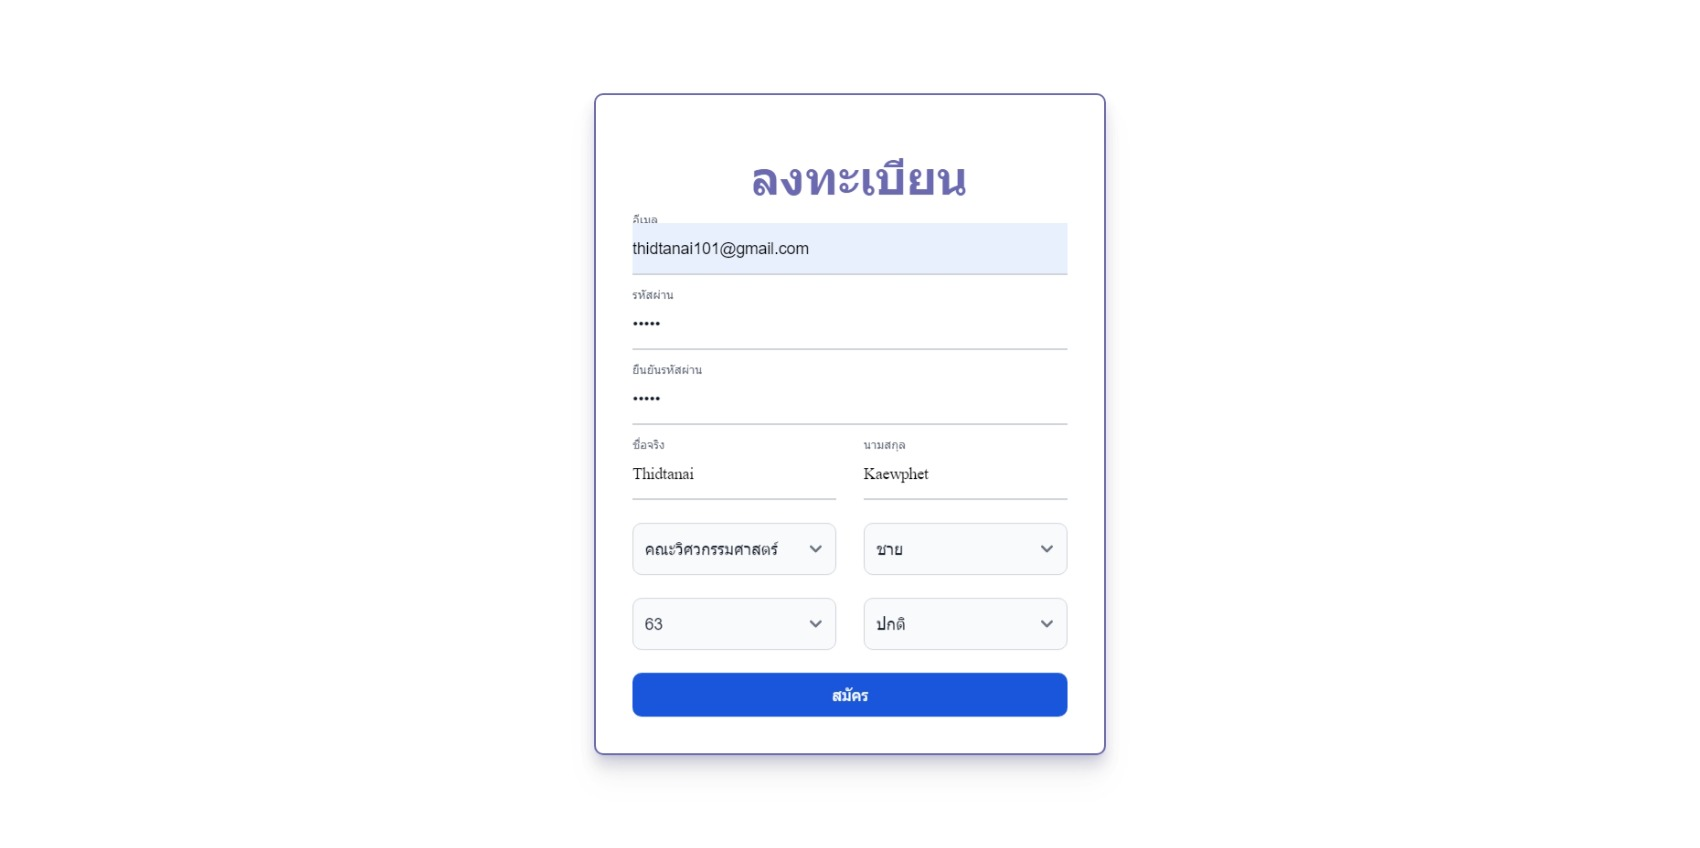
\includegraphics[width=\linewidth]{image/web/register.jpeg}
    \caption{หน้าล็อกลงทะเบียน}
  \end{subfigure}
  \hfill
  \begin{subfigure}[b]{0.4\linewidth}
    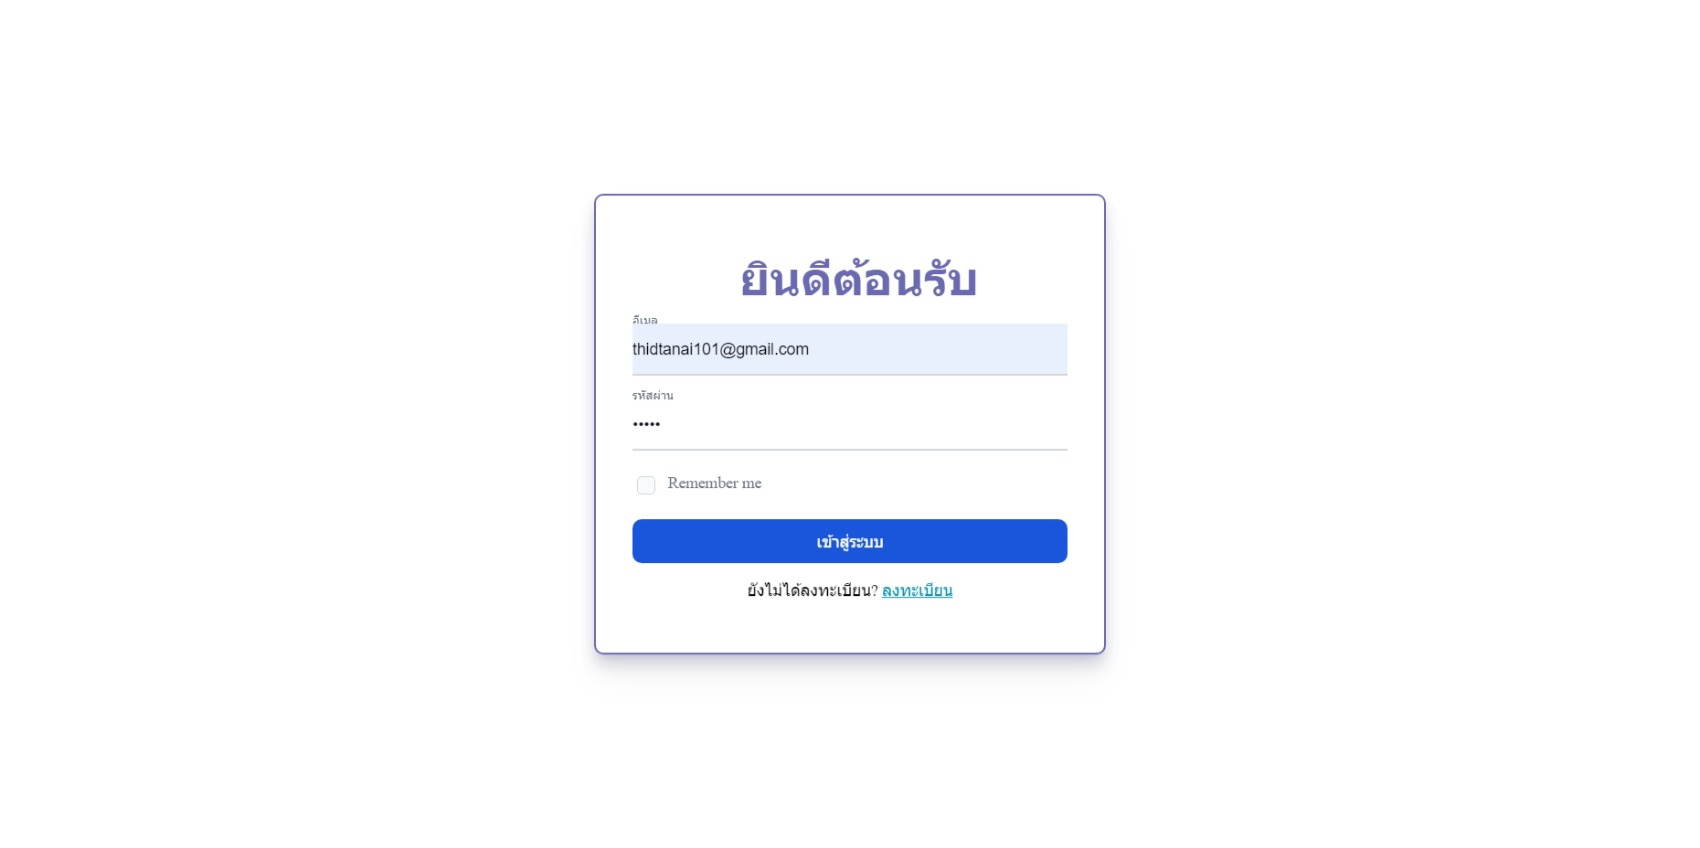
\includegraphics[width=\linewidth]{image/web/login.jpeg}
    \caption{หน้าเข้าสู่ระบบ}
  \end{subfigure}
  \caption{ผลการลงทะเบียนและการเข้าสู่ระบบ}
  \label{fig:register-login}
\end{figure}

\subsection{ระบบเลือกความสนใจ}
มีหน้าเลือกความสนใจแสดงขึ้นมาให้ผู้ใช้หากผู้ใช้เข้าสู่ระบบเป็นครั้งแรก
\begin{figure}[h] 
    \begin{center}
        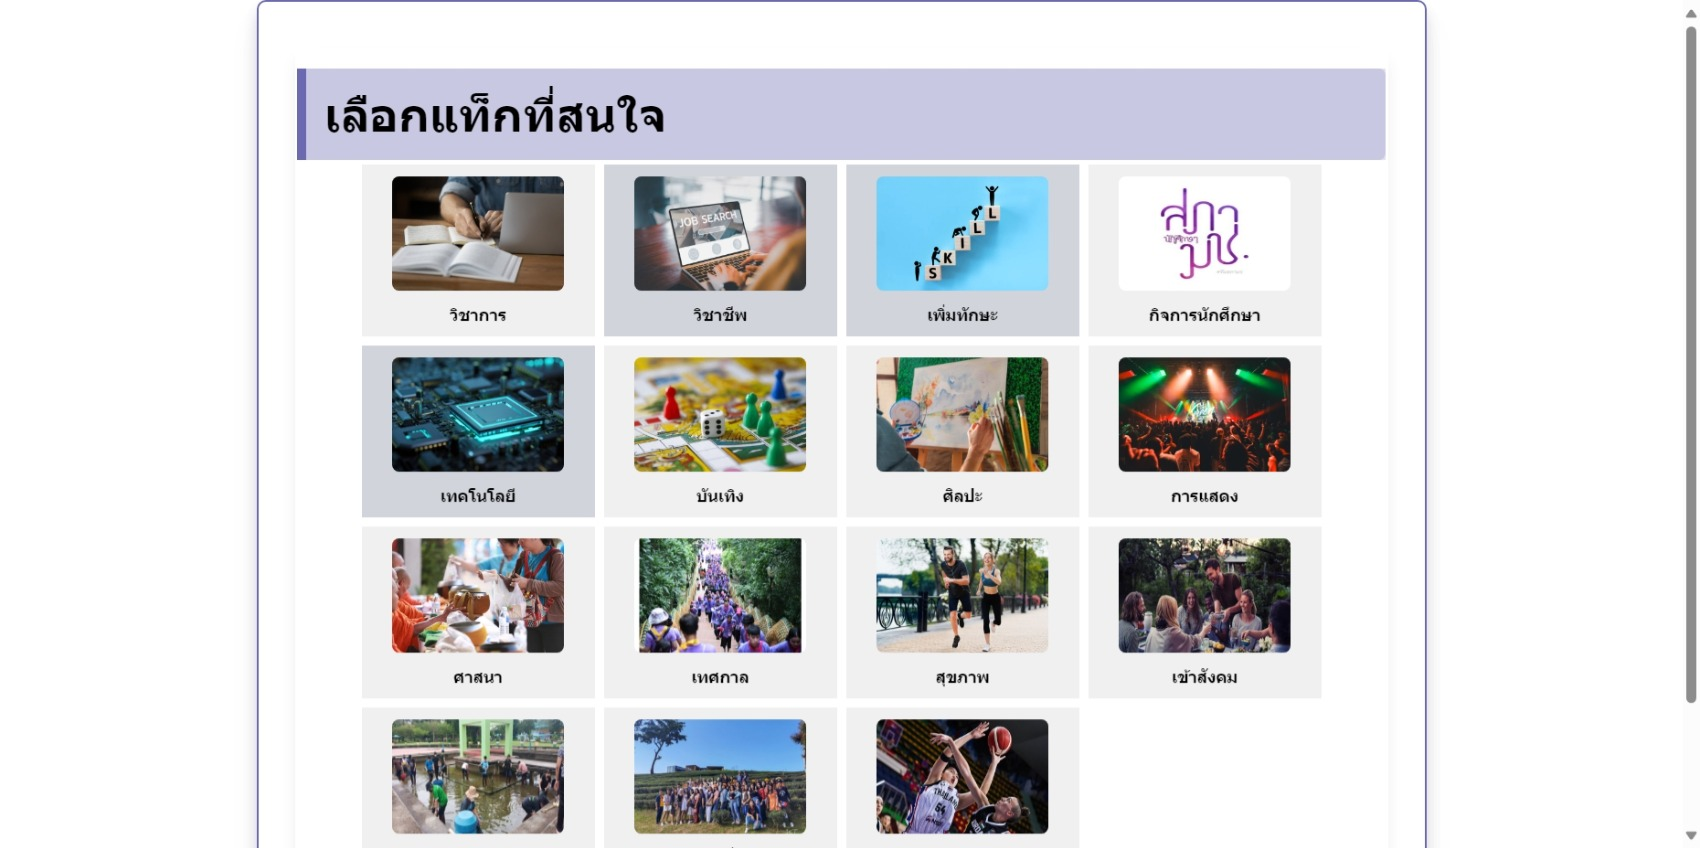
\includegraphics[width=0.6\linewidth]{image/web/choose.jpeg}
    \end{center}
    \caption{ผลการแสดงหน้าเลือกความสนใจหลังเข้าสู่ระบบครั้งแรก}
    \label{fig:choose}
\end{figure}

\newpage

\subsection{การแสดงผลระหว่างผู้ใช้ที่เข้าสู่ระบบแล้วกับยังไม่ได้เข้าสู่ระบบ}
ผู้ใช้ที่ไม่ได้เข้าสู่ระบบจะสามารถดูได้แค่หน้าหลักและหน้าข่าวสารกิจกรรม ส่วนผู้ใช้ที่เข้าสู่ระบบแล้วจะสามารถเข้าถึงหน้าต่างๆได้เพิ่มขึ้น
\begin{figure}[h]
  \centering
  \begin{subfigure}[b]{0.4\linewidth}
    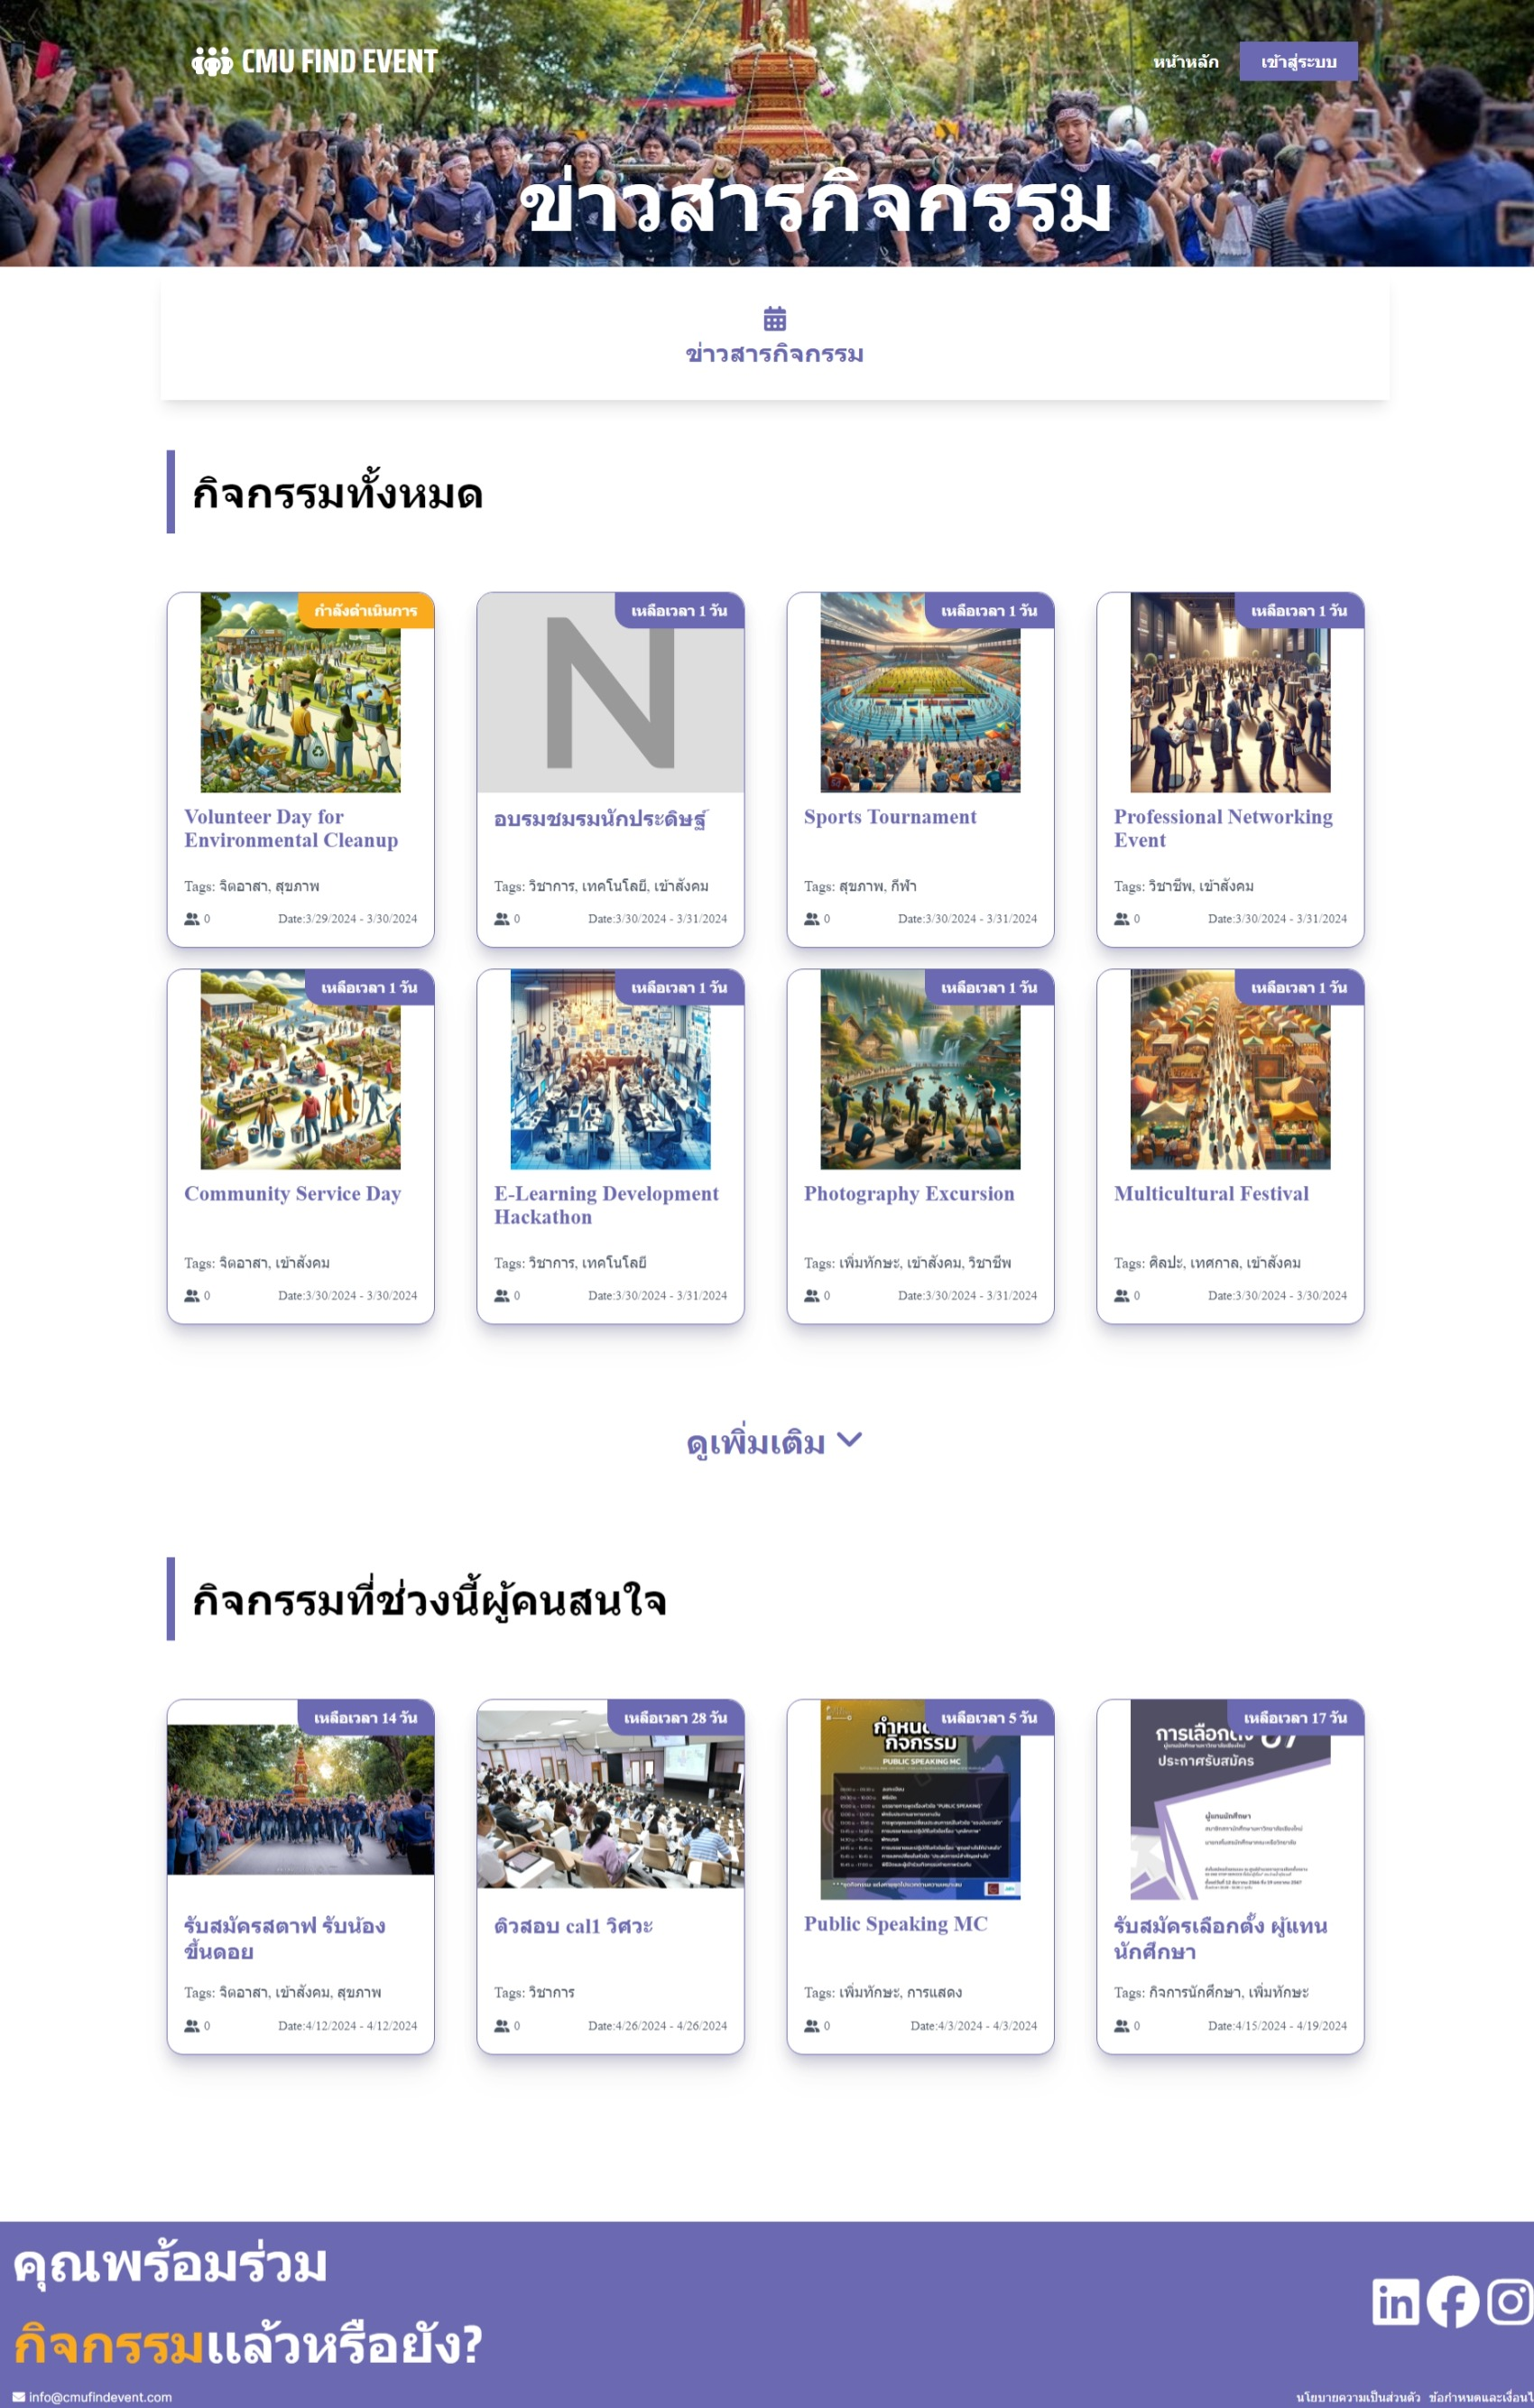
\includegraphics[width=\linewidth]{image/web/notLog-activity.jpeg}
    \caption{หน้าข่าวสารกิจกรรมของผู้ใช้ที่ยังไม่ได้เข้าสู่ระบบ}
  \end{subfigure}
  \hfill
  \begin{subfigure}[b]{0.4\linewidth}
    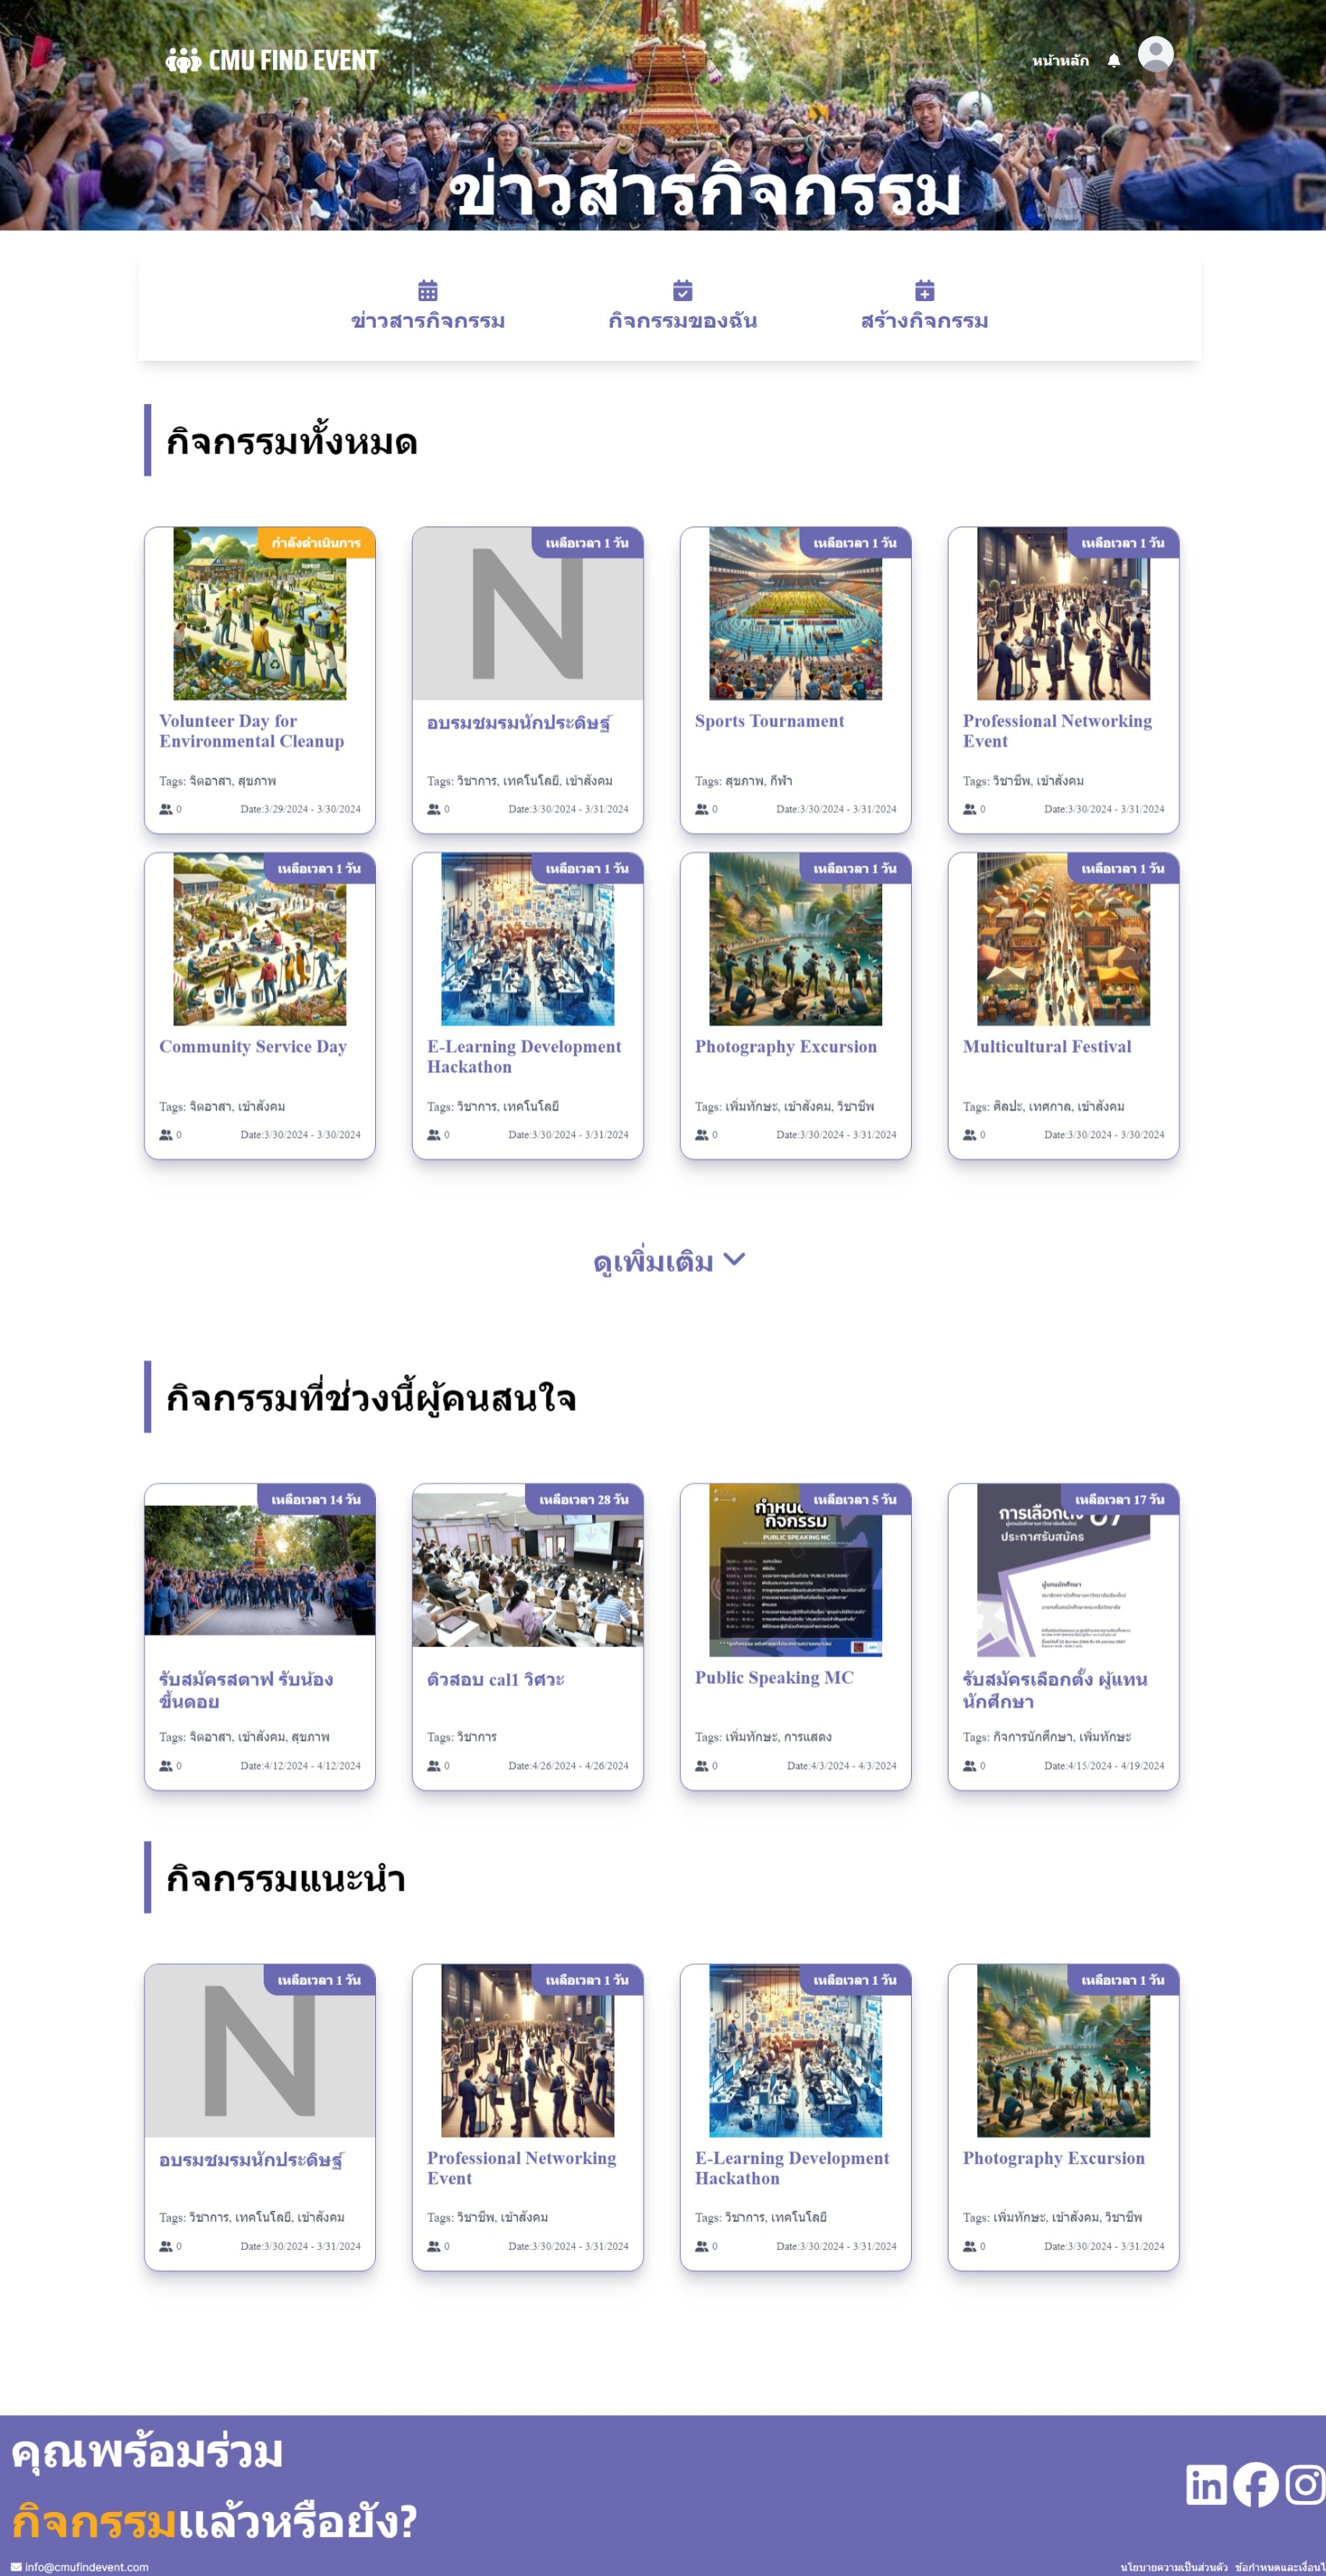
\includegraphics[width=\linewidth]{image/web/activity.jpeg}
    \caption{หน้าข่าวสารกิจกรรมของผู้ใช้ที่เข้าสู่ระบบแล้ว}
  \end{subfigure}
  \caption{ผลการแสดงผลระหว่างผู้ใช้ที่เข้าสู่ระบบแล้วกับยังไม่ได้เข้าสู่ระบบ}
  \label{fig:loginShow}
\end{figure}

\FloatBarrier

\newpage
\subsection{ระบบแนะนำกิจกรรมที่ผู้ใช้อาจสนใจ}
หลังจากที่ผู้ใช้เลือกแท็กกิจกรรมที่สนใจแล้วจะมีส่วนของกิจกรรมที่แนะนำแสดงเพิ่มขึ้นมา โดยกิจกรรมที่แนะนำนั้นจะตรงกับแท็กที่ผู้ใช้เลือก
\begin{figure}[h]
  \centering
  \begin{subfigure}[b]{0.4\linewidth}
    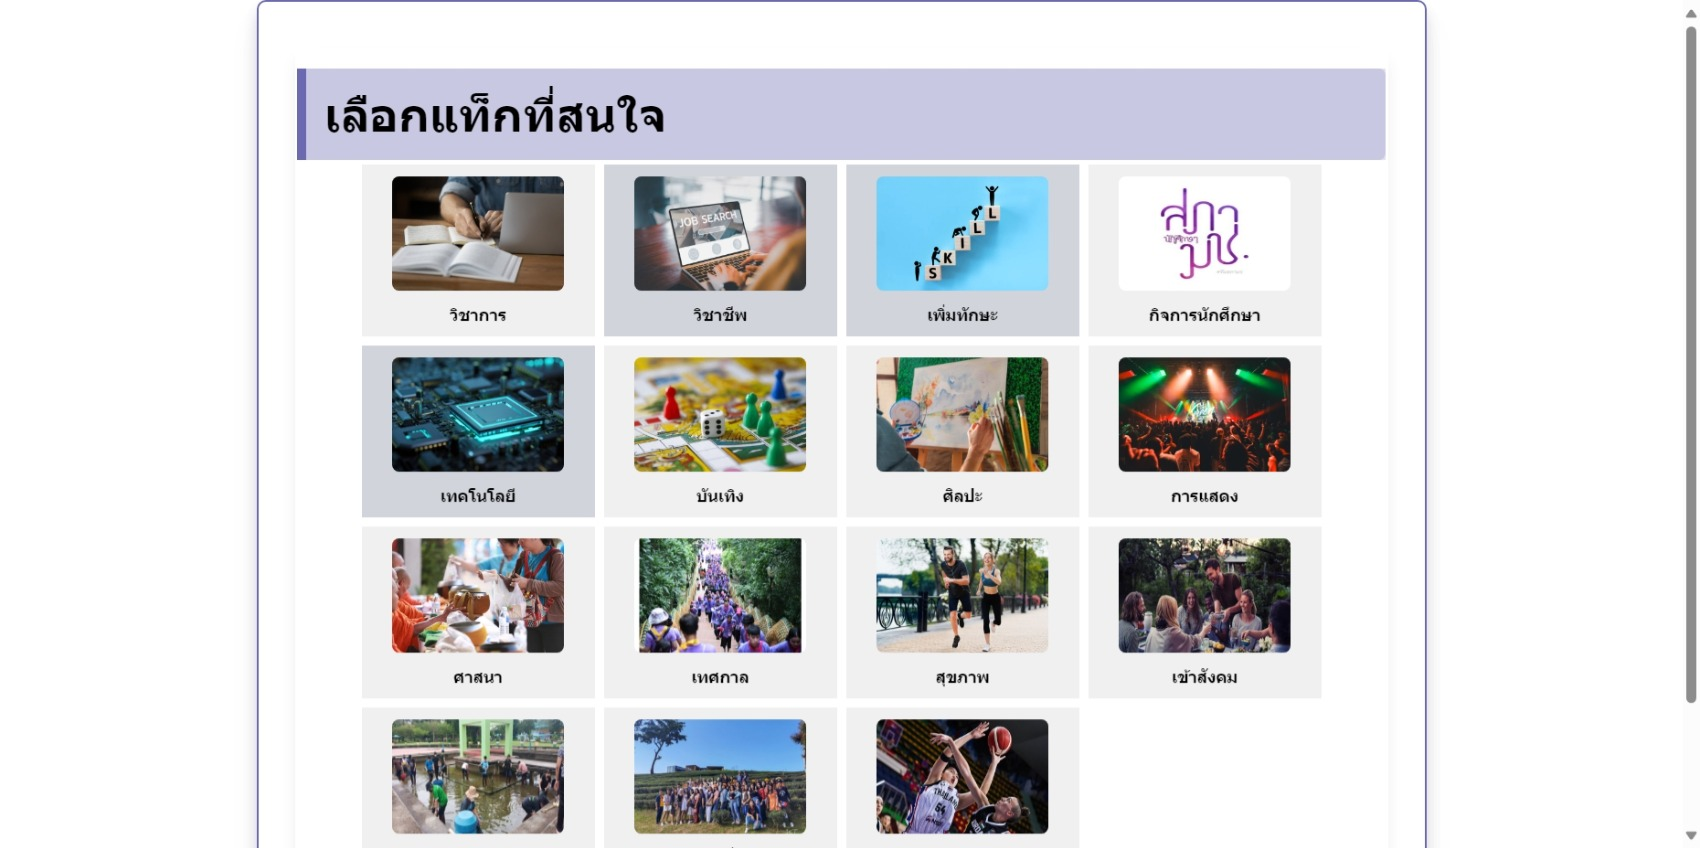
\includegraphics[width=\linewidth]{image/web/choose.jpeg}
    \caption{แท็กกิจกรรมที่ผู้ใช้เลือก}
  \end{subfigure}
  \hfill
  \begin{subfigure}[b]{0.4\linewidth}
    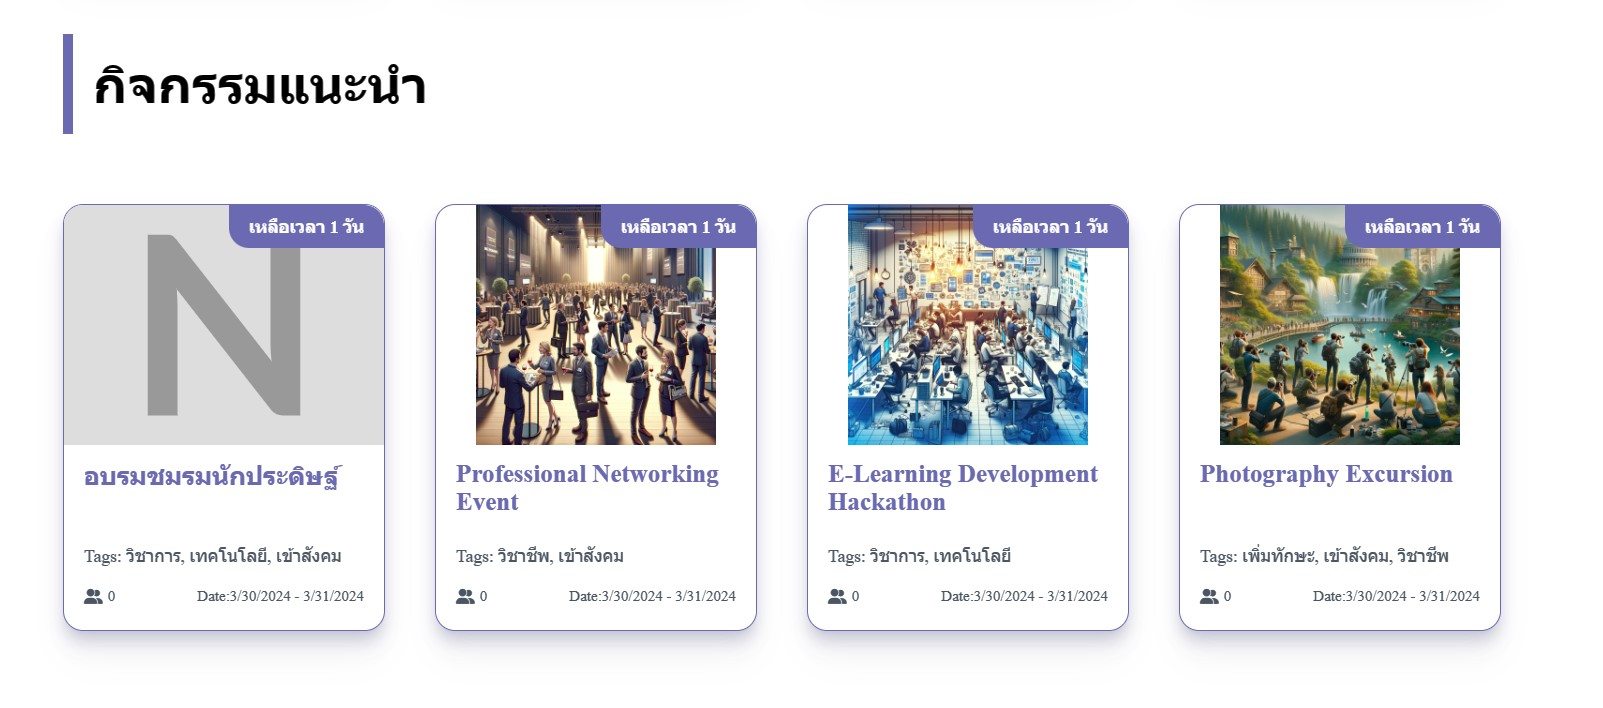
\includegraphics[width=\linewidth]{image/web/recommend.jpg}
    \caption{กิจกรรมที่แนะนำให้กับผู้ใช้}
  \end{subfigure}
  \caption{ผลแนะนำกิจกรรมที่ผู้ใช้อาจสนใจ}
  \label{fig:reccomended}
\end{figure}

\FloatBarrier

\subsection{ระบบประกาศกิจกรรม}
ผู้ใช้สามารถสร้างกิจกรรมขึ้นมาใหม่ได้ และสามารถเลือกได้ว่าจะเปิดรับสมัครตำแหน่งอะไรด้วยไหมได้ โดยหลังจากสร้างกิจกรรมแล้ว กิจกรรมนั้นจะถูกประกาศในหน้าประกาศกิจกรรมโดยมีข้อมูลแสดงถูกต้อง
\begin{figure}[h]
  \centering
  \begin{subfigure}[b]{0.4\linewidth}
    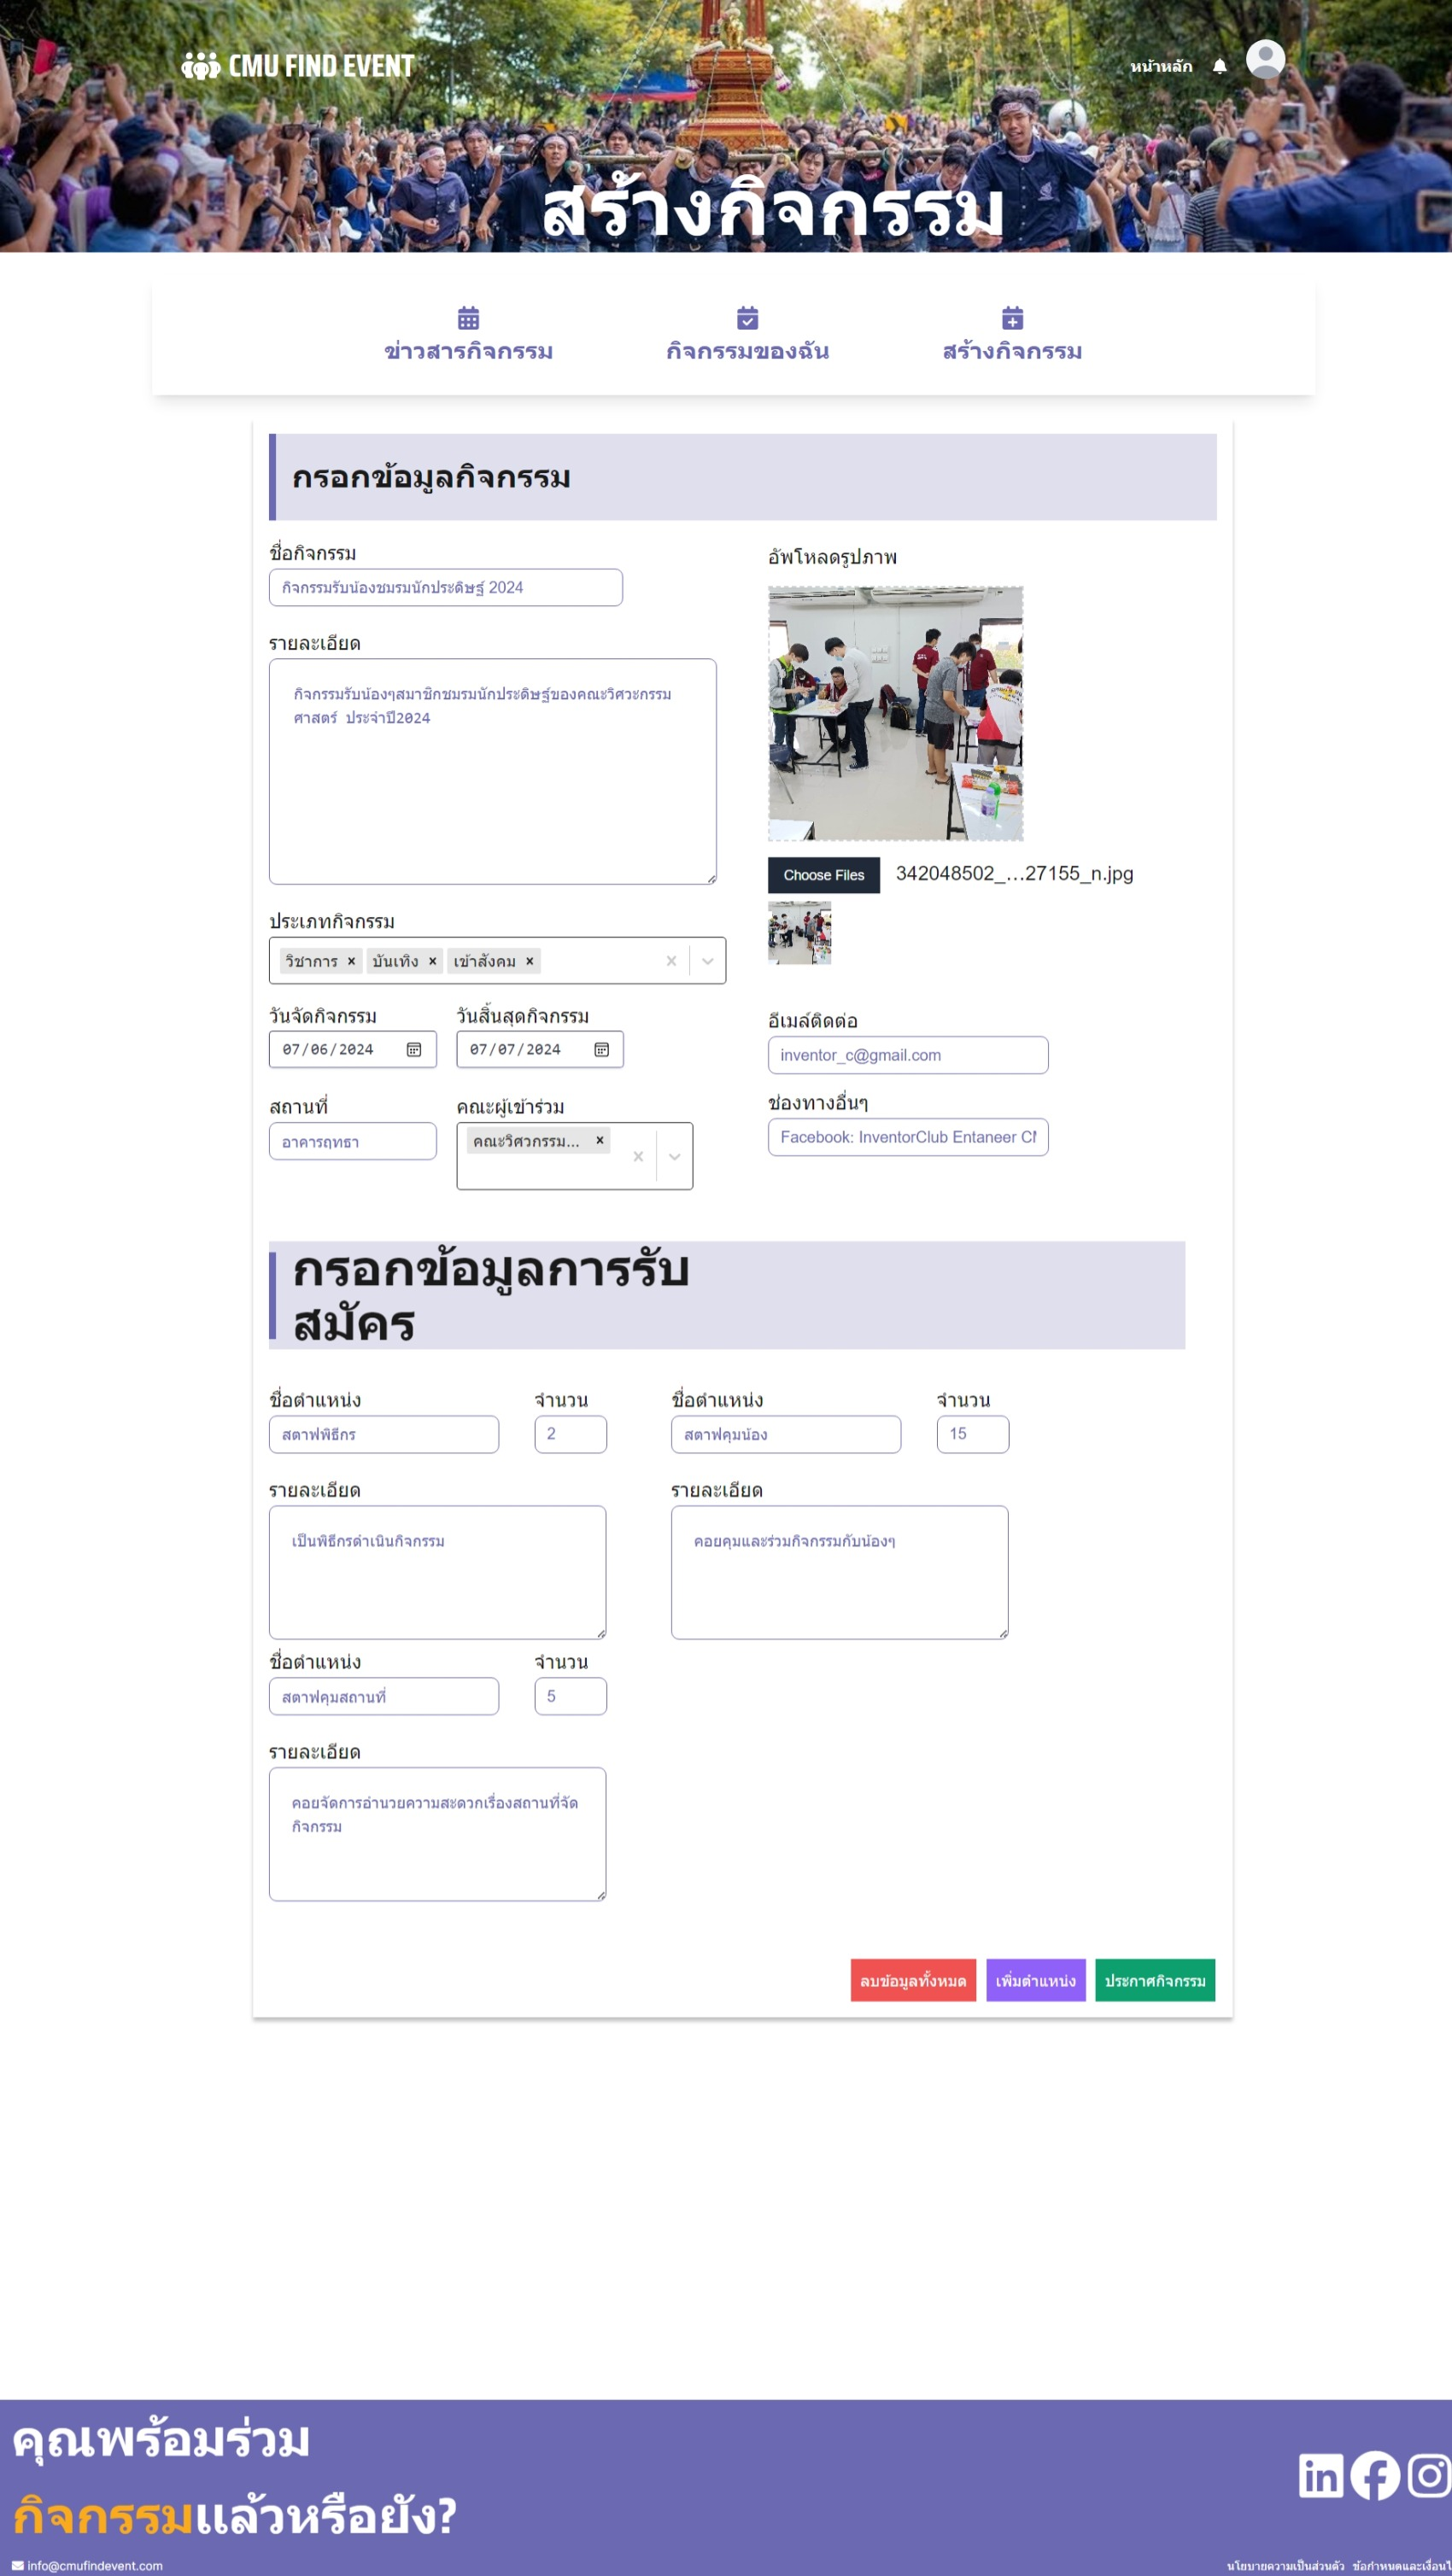
\includegraphics[width=\linewidth]{image/web/create.jpeg}
    \caption{หน้าสร้างกิจกรรม}
  \end{subfigure}
  \hfill
  \begin{subfigure}[b]{0.4\linewidth}
    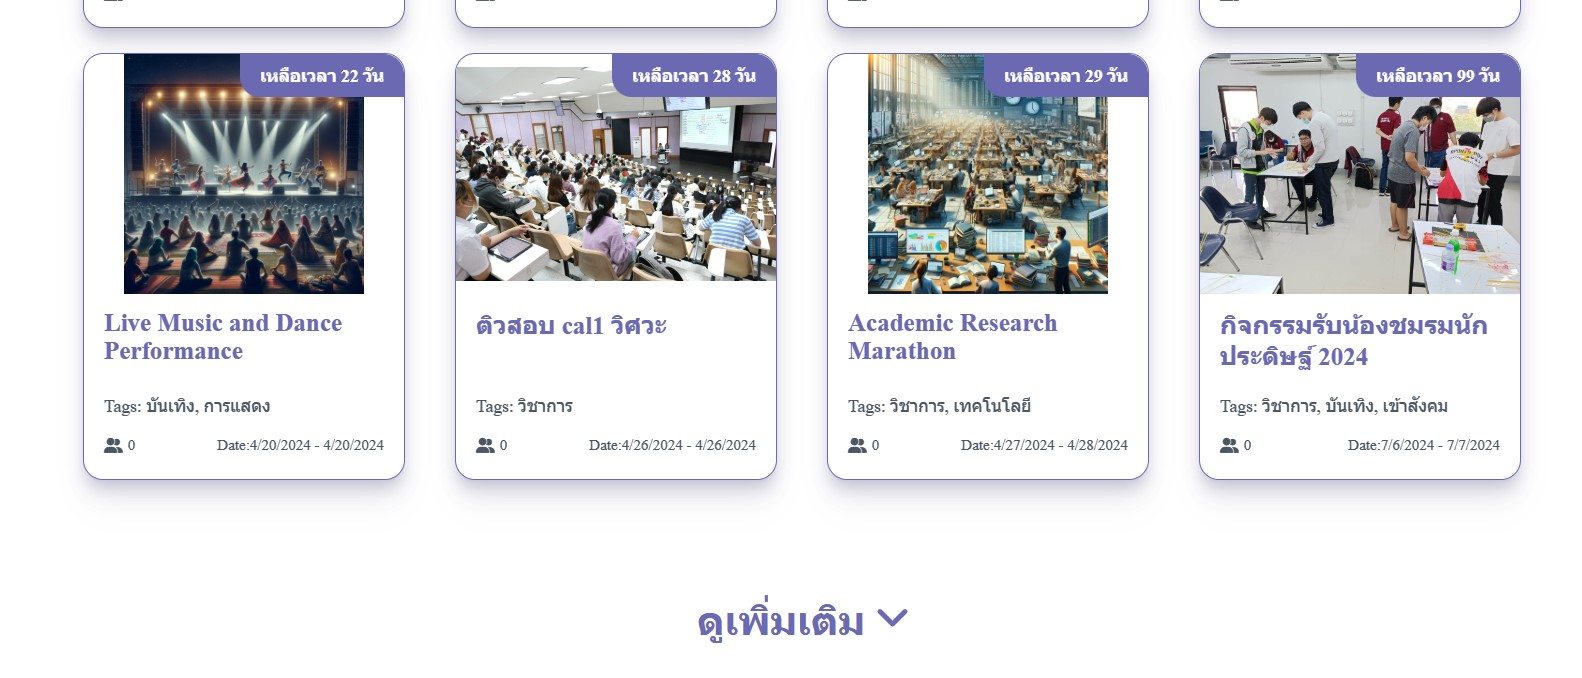
\includegraphics[width=\linewidth]{image/web/showCreate.jpg}
    \caption{กิจกรรมถูกประกาศหลังจากที่ถูกสร้างแล้ว}
  \end{subfigure}
  \caption{ผลการประกาศกิจกรรม}
  \label{fig:create}
\end{figure}

\FloatBarrier

\subsection{ระบบกิจกรรมของฉัน}
หลังจากที่ผู้ใช้กดสนใจกิจกรรมหรือสมัครเข้าร่วมกิจกรรมใดๆ กิจกรรมนั้นๆจะถูกแสดงในหน้ากิจกรรมของฉัน
\begin{figure}[h]
  \centering
  \begin{subfigure}[b]{0.4\linewidth}
    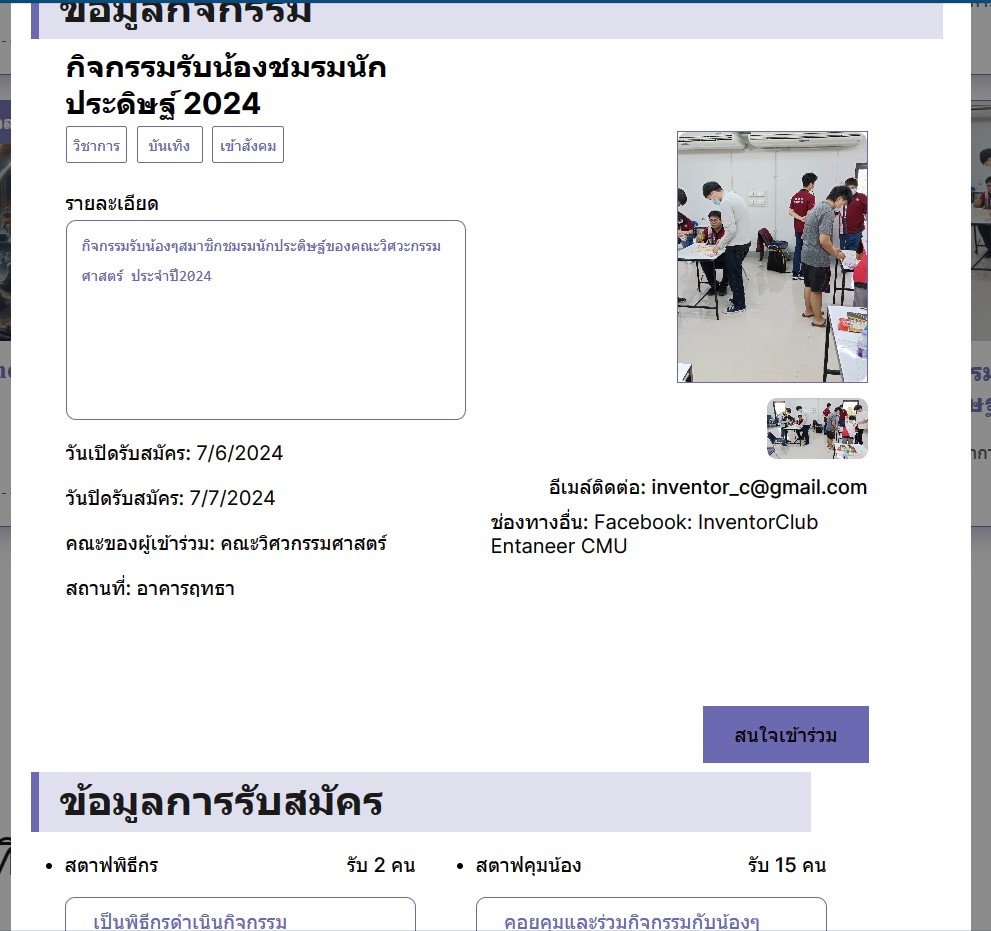
\includegraphics[width=\linewidth]{image/web/showInfo.jpg}
    \caption{กดสนใจกิจกรรม}
  \end{subfigure}
  \hfill
  \begin{subfigure}[b]{0.4\linewidth}
    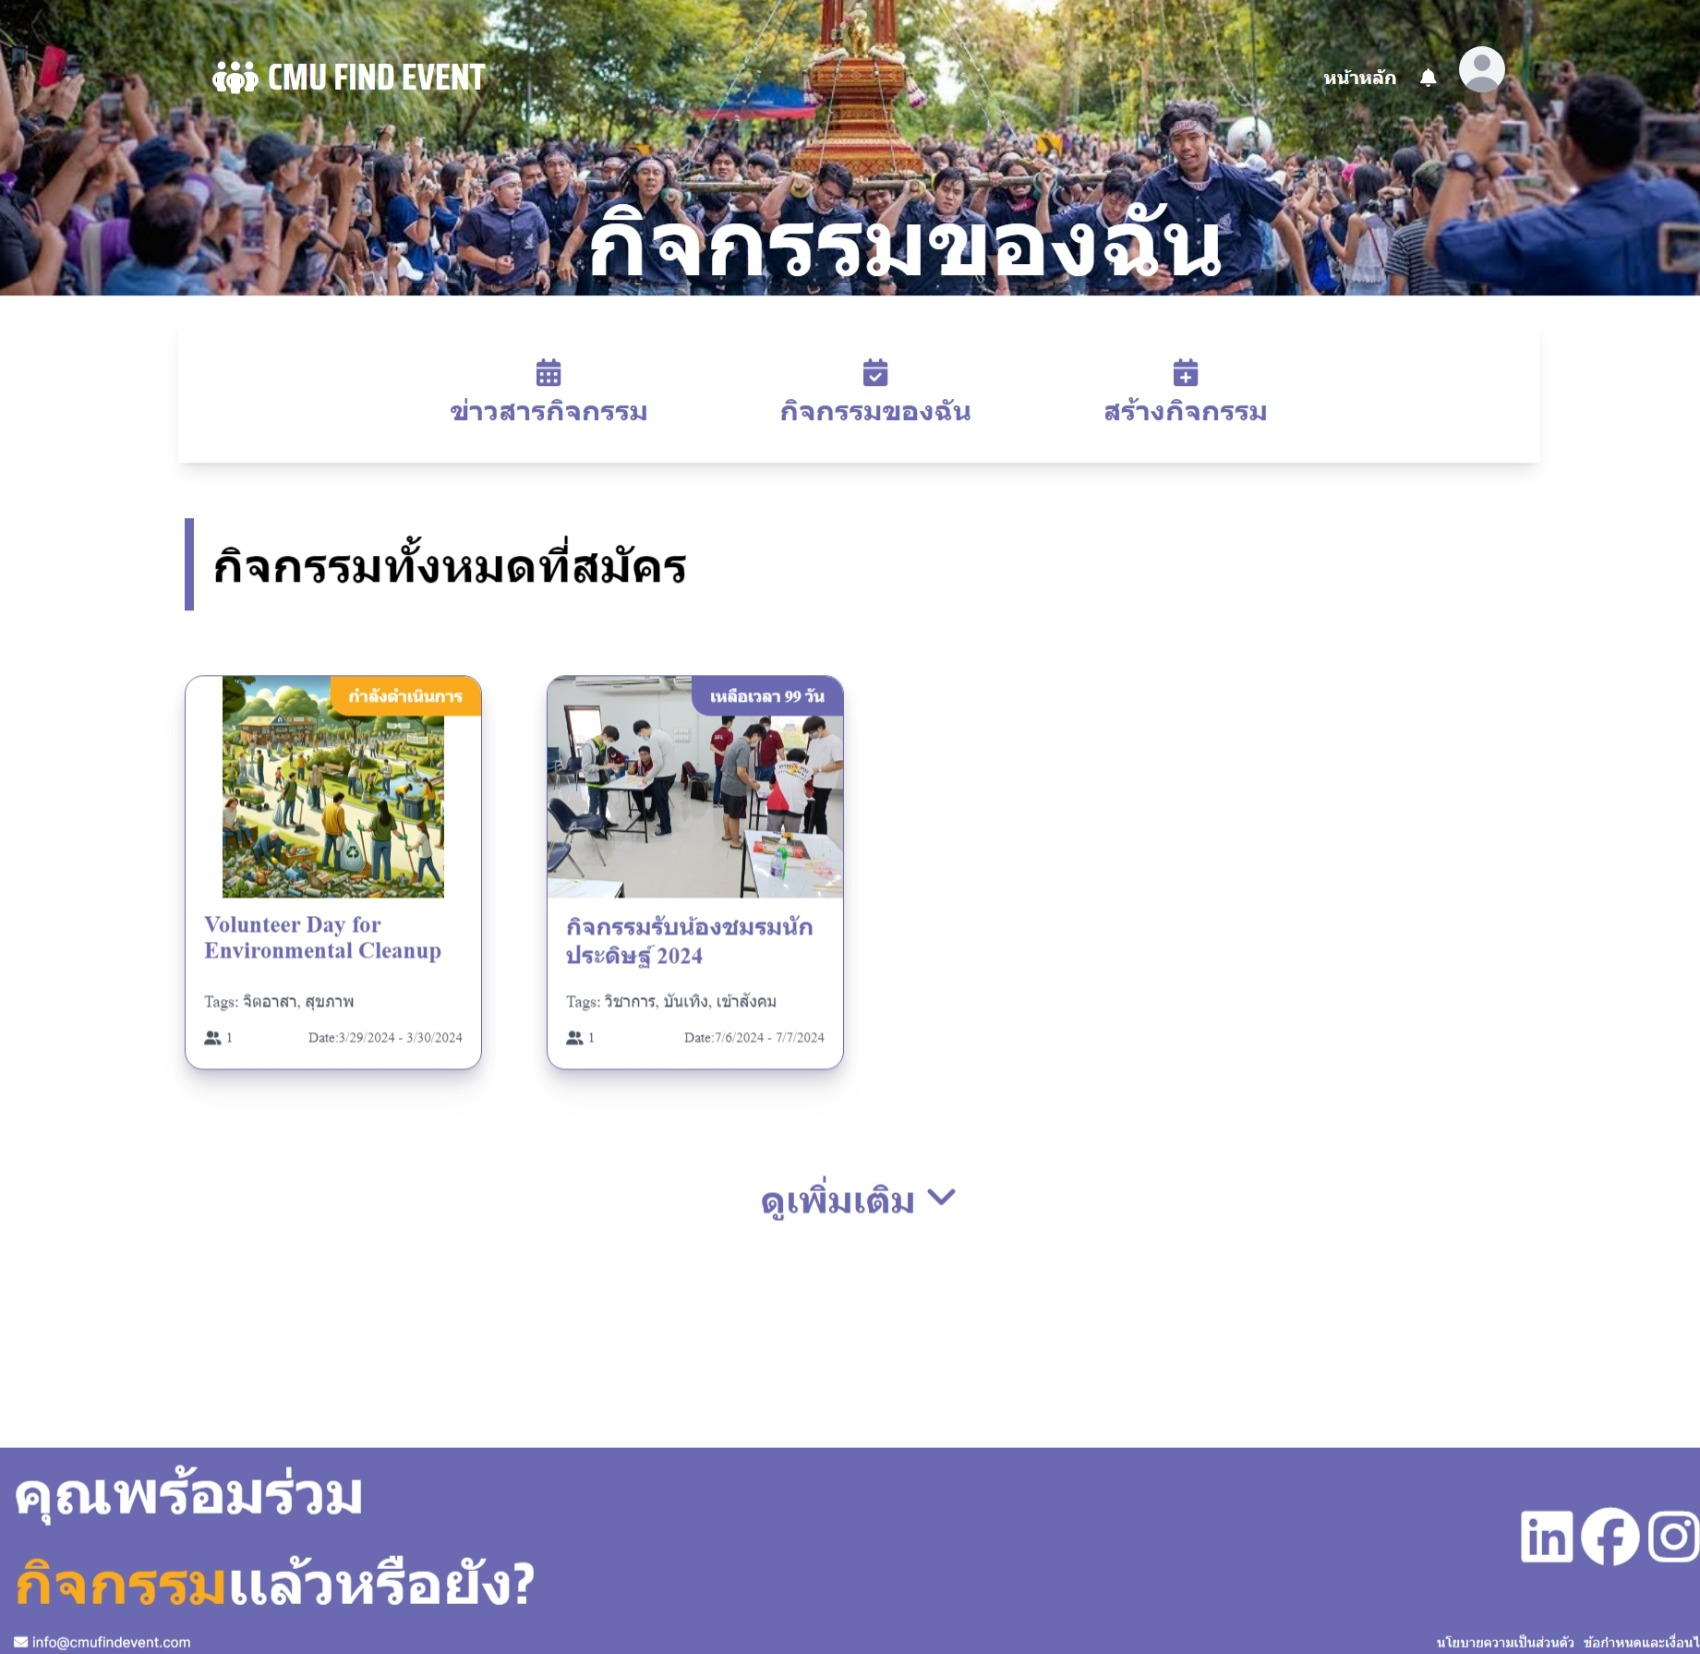
\includegraphics[width=\linewidth]{image/web/myAct.jpeg}
    \caption{กิจกรรมถูกแสดงในหน้ากิจกรรมของฉัน}
  \end{subfigure}
  \caption{ผลการกดสนใจกิจกรรม}
  \label{fig:interests}
\end{figure}

\FloatBarrier

\subsection{ระบบสมัครตำแหน่งในกิจกรรม}
หลังจากที่ผู้ใช้กดสมัครกิจกรรมในตำแหน่งที่สนใจไป จะมีหน้าต่างให้กรอกคำขอสมัคร หลังจากกดส่งคำขอสมัครแล้ว คำขอจะส่งถูกส่งไปยังผู้สร้างกิจกรรมนั้นๆโดยผู้ใช้จะสามารถดูคำขอต่างๆได้จากปุ่มกระดิ่งแจ้งเตือน อีกทั้งยังสามารถตอบรับหรือปฏิเสธคำขอได้
\begin{figure}[h]
  \centering
  \begin{subfigure}[b]{0.4\linewidth}
    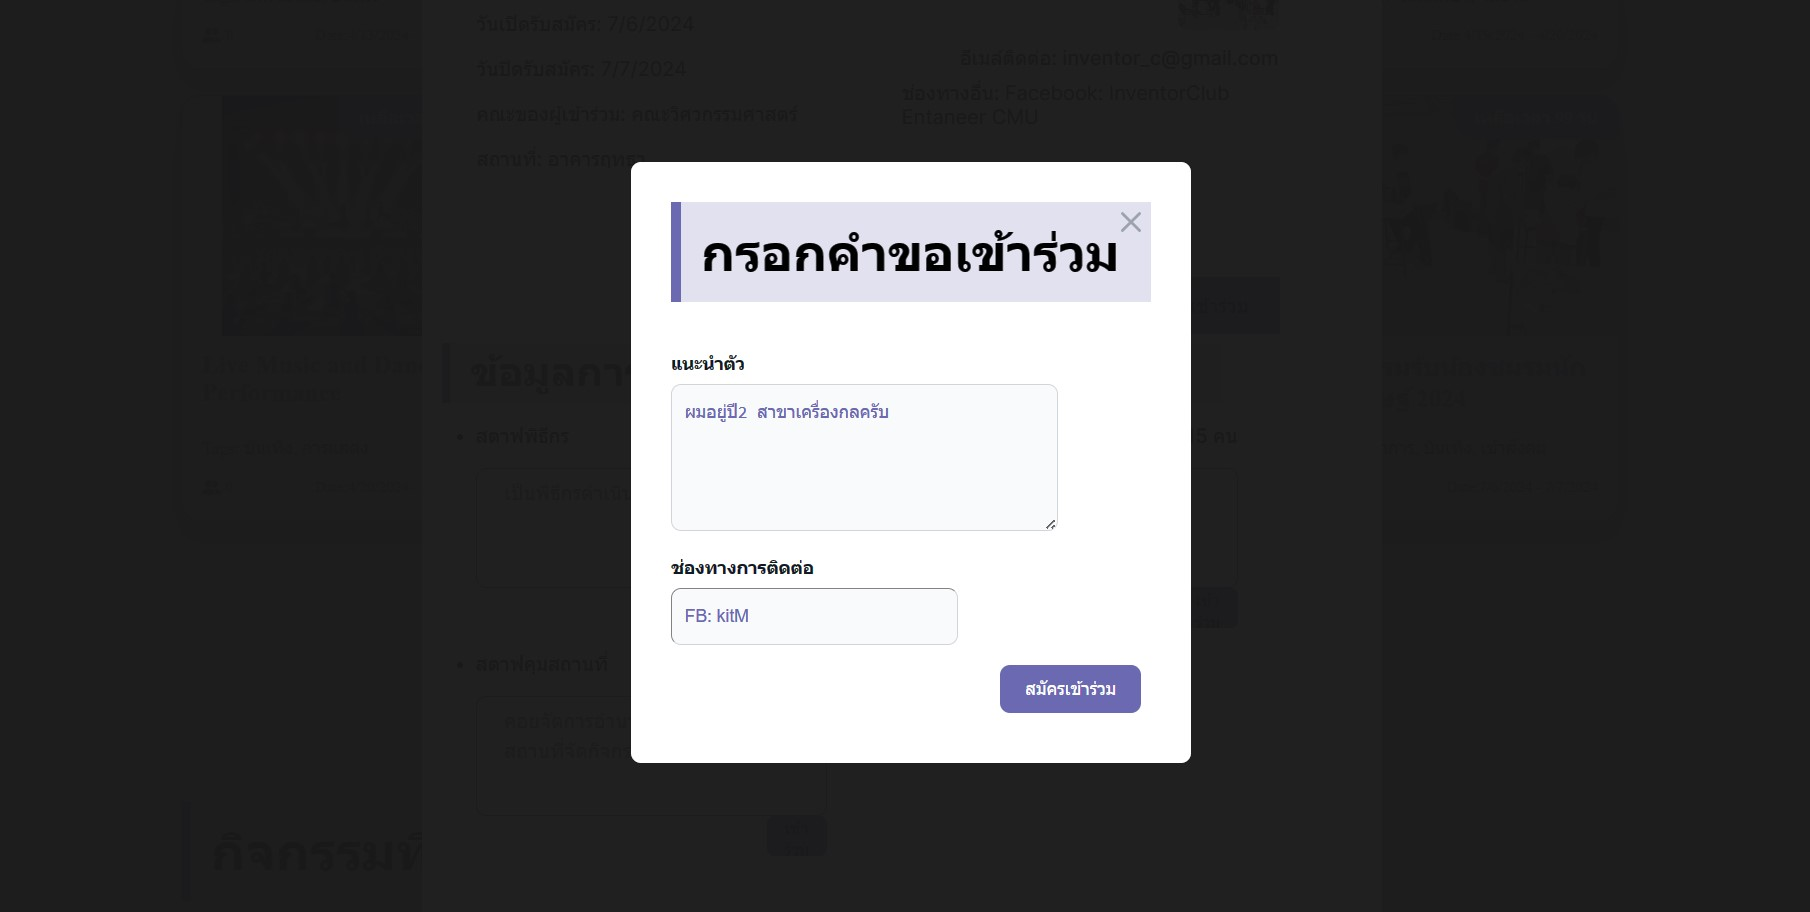
\includegraphics[width=\linewidth]{image/web/createReq.jpg}
    \caption{ผู้ใช้กรอกข้อมูลสมัครตำแหน่งของกิจกรรมไป}
  \end{subfigure}
  \hfill
  \begin{subfigure}[b]{0.4\linewidth}
    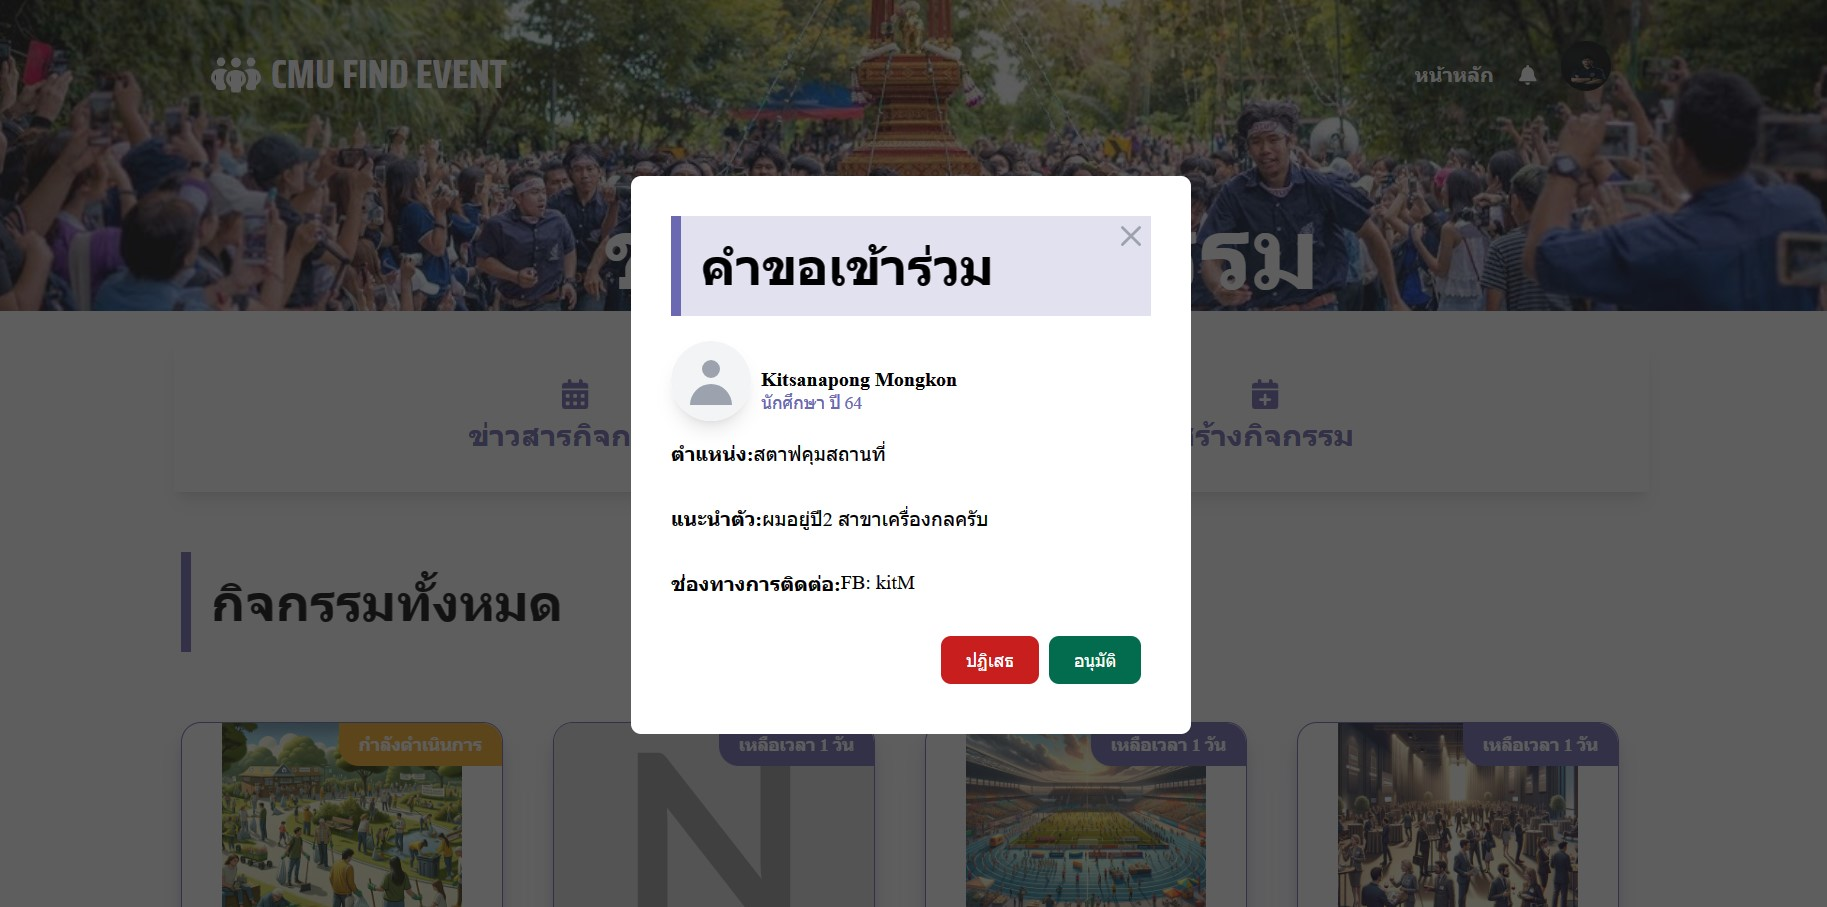
\includegraphics[width=\linewidth]{image/web/joinReq.jpg}
    \caption{ผู้สร้างกิจกรรมเห็นคำขอสมัครเข้าร่วม}
  \end{subfigure}
  \caption{ผลระบบสมัครตำแหน่งในกิจกรรม}
  \label{fig:joinReq}
\end{figure}

\FloatBarrier